\documentclass[IB,BIB]{TFUOC}%IB: CASTELLANO, CAT: CATALÁN, ENG: ANGLÈS

%Introducción de datos del trabajo
\title{Título del trabajo completo y tan largo como sea necesario}
\titcrt{Título muy corto} %Título corto que aparecerá a la cabecera
\author{Nombre Estudiando Estudiante}
\date{21 de septiembre de 2021}


\nomPDC{Nombre Tutor Tutora}
\nomPRA{Nombre Profesorado Responsable}
\titulac{Máster en XXX}
\area{Área del trabajo}
\idioma{Castellano}
\credits{15}
\parcla{palabra, clave, trabajo}

\licenc{ccBy}
%Posibles licencias
%ccByNcNd
%ccByNcSa
%ccByNc
%ccByNd
%ccBySa
%ccBy
%GNU
%copyright


%%%%%%%%%%
% Resumen en el idioma

\abstractidioma{
Máximo 250 palabras, con la finalidad, contexto de aplicación, metodología, resultados y conclusiones del trabajo.
}

% Resumen en inglés.
\abstractenglish{
A maximum of 250 words, detailing the purpose, contexto of application, methodology, results and conclusiones of the work.
}

\begin{document}

\estructura

\tableofcontents

\listoffigures

\listoftables




\chapter{Introducción}

Esta plantilla se concibe como una guía para el estudiante. Se puede adaptar a las necesidades de cada trabajo, siempre que el/la tutor/a del trabajo esté de acuerdo..

\section{Contexto y justificación del trabajo}


Punto de partida del trabajo (¿Cuál es la necesidad a cubrir? ¿Por qué es un tema relevante? ¿Cómo se resuelve el problema de momento?) y aportación realizada (¿Qué resultado se quiere obtener?).

Es importante tener en cuenta que el trabajo final tiene que ser comprensible para cualquier persona que conozca el área de conocimiento, pero no tiene porque ser experta en el tema del que versa el trabajo.

\section{Objetivos del trabajo}

Listado de los objetivos del trabajo.

\section{Impacto en sostenibilidad, ético-social y de diversidad}
\label{s:etic}

Esta sección tendría que identificar los impactos positivos y/o negativos del trabajo final en las tres dimensiones de la competencia transversal UOC “Compromiso ético y global”.
 
La Guía transversal sobre la Competencia Ética y Global os ayudará a redactar estos apartados.


\section{Enfoque y método seguido}

Mención de cuáles son las posibles estrategias para llevar a cabo el trabajo y cuál es la estrategia elegida (desarrollar un producto nuevo, adaptar un producto existente...). Hay que incluir una valoración de por qué esta es la estrategia más apropiada para conseguir los objetivos.   	



\section{Planificación del trabajo}

Descripción de los recursos necesarios para hacer el trabajo, las tareas a realizar y una planificación temporal de cada tarea mediante un diagrama de Gantt o similar. Esta planificación tendría que marcar cuáles son los hitos parciales de cada una de las PEC.

Identificación de los posibles riesgos que pueden hacer que esta planificación no se cumpla y descripción de los planes de mitigación o alternativos en caso de que estos riesgos sean un problema.


\section{Breve sumario de productos obtenidos}

No hay que entrar en detalle: la descripción detallada se hará en el resto de capítulos.


\section{Breve descripción de los otros capítulos de la memoria}

Breve explicación de los contenidos de cada capítulo y su relación con el proyecto global.

\chapter{Estado del arte}

Estado del arte del tema en cuestión.
Tendría que acabar mostrando por qué el trabajo es importante y que aporta algo, y con las hipótesis del trabajo.


En estos apartados, hay que describir:
\begin{itemize}
    \item Los aspectos más relevante del diseño y desarrollo del trabajo.
    \item La metodología elegida para hacer este desarrollo, describiendo las alternativas posibles, las decisiones tomadas, y los criterios utilizados para tomar estas decisiones.
    \item Los productos obtenidos.
\end{itemize}




\chapter{Resultados}

Detallad en este apartado los resultados obtenidos utilizando la metodología descrita en el apartado anterior.


%Compilación de los resultados del trabajo. Tendría que haber una correspondencia con la metodología en el sentido que los resultados es el que se obtiene después de haber aplicado la metodología.

Las figuras tienen que estar explicadas y citadas en el texto, como la \ref{fig:my_label}, en la cual se muestra el error en función de la distancia, en unidades arbitrarias. En todas las gráficas tiene que haber el título de los ejes.

\begin{figure}[!htbp]
    \centering
    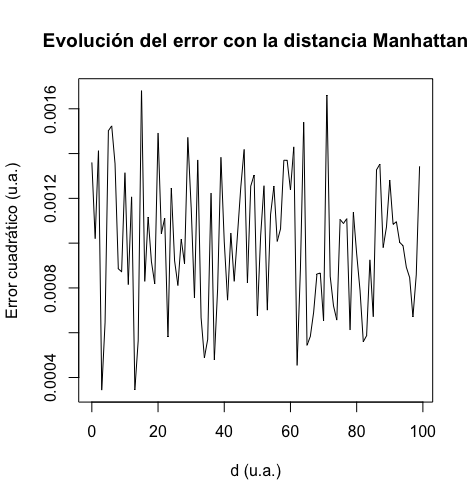
\includegraphics[width=7truecm]{Rplotmanh.png}
    \caption{Error en función de la distancia en unidades arbitrarias.}
    \label{fig:my_label}
\end{figure}
 
\textbf{La estructuración de los capítulos puede variar según el tipo de trabajo.}  
 
En caso de que se proceda, se incluirá un apartado de “Valoración económica del trabajo”. Este apartado indicará los gastos asociados al desarrollo y mantenimiento del trabajo, así como los beneficios económicos obtenidos y un análisis final sobre la viabilidad del producto.



\chapter{Resultados}

Detallad en este apartado los resultados obtenidos utilizando la metodología descrita en el apartado anterior.

Las figuras tienen que estar explicadas y citadas en el texto, como la \ref{fig:my_label}, en la cual se muestra el error en función de la distancia, en unidades arbitrarias. En todas las gráficas tiene que haber el título de los ejes.

\begin{figure}[!htbp]
    \centering
    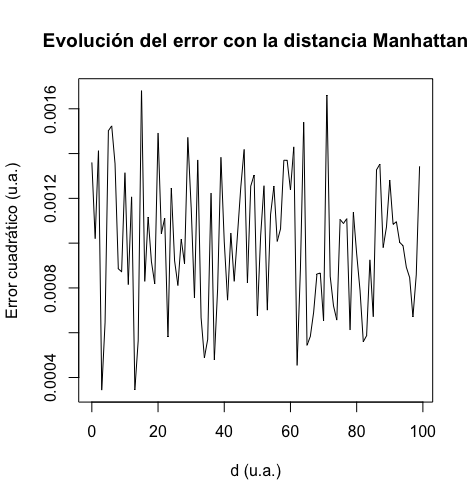
\includegraphics[width=7truecm]{Rplotmanh.png}
    \caption{Error en función de la distancia en unidades arbitrarias.}
    \label{fig:my_label}
\end{figure}

\chapter{Discusión}
Discusión de los resultados en el contexto del proyecto. Es en este apartado donde cobran sentido y en el cual se responden las preguntas de investigación y se muestra cómo los resultados dan respuesta a los problemas planteados.

Esta parte puede ser que no aplique según el tipo de trabajo.

\chapter{Valoración económica}
En caso de que corresponda, se incluirá un apartado de ``Valoración económica del trabajo". Este apartado indicará los gastos asociados al desarrollo y mantenimiento del trabajo, así como los beneficios económicos obtenidos. Hay que hacer un análisis final sobre la viabilidad del producto.

\chapter{Conclusiones y trabajos futuros}

\section{Conclusiones}
Este capítulo tiene que incluir:
\begin{itemize}
\item Una descripción de las conclusiones del trabajo:
\begin{itemize}
    \item Una vez se han obtenido los resultados, ¿qué conclusiones se extraen?
    \item ¿Estos resultados son los esperados? ¿O han sido sorprendentes? ¿Por qué? 
\end{itemize}
\item Una reflexión crítica sobre el logro de los objetivos planteados inicialmente:
\begin{itemize}
    \item ¿Hemos logrado todos los objetivos? Si la respuesta es negativa, ¿por qué motivo?
\end{itemize}
\end{itemize}


\section{Líneas de futuro}
Las líneas de trabajo futuro que no se han podido explorar en este trabajo y han quedado pendientes.

\section{Seguimiento de la planificación}


\begin{itemize}
\item 
Un análisis crítico del seguimiento de la planificación y metodología a lo largo del producto:
\begin{itemize}
    \item ¿Se ha seguido la planificación?
    \item ¿La metodología prevista ha sido suficientemente adecuada?
    \item ¿Ha habido que introducir cambios para garantizar el éxito del trabajo? ¿Por qué? 
\end{itemize}
\item De los impactos previstos a \ref{s:etic}, ético-sociales, de sostenibilidad y de diversidad, avaluad/mencionad si se han mitigado (si eran negativos) o si se han conseguido (si eran positivos). 
\item Si han aparecido impactos no previstos en \ref{s:etic}, evaluar/mencionar cómo se han mitigado (si eran negativos) o que han aportado (si eran positivos).
\end{itemize}


\chapter{Glosario}

Definición de los términos y acrónimos más relevantes utilizados dentro de la Memoria.


\chapter{Bibliografía}

Lista numerada de las referencias bibliográficas utilizadas dentro de la memoria. En cada lugar donde se utilice una referencia dentro del texto, se tiene que indicar citando el número de la referencia, por ejemplo: [7].

Es muy importante incluir todas las referencias utilizadas y citarlas apropiadamente, es decir, incluyendo toda la información necesaria para identificar la referencia. La información mínima que se tiene que incluir según el tipo de referencia es:

\begin{itemize}
\item Libro: Autores, Título, Edición (si procede) Editorial, Ciudad, Año.
\item  Artículo de revista: Autores, Título, Nombre de la Revista, Número de Página inicial y final, Número de la revista / Volumen, Año.
\item  Web: URL y fecha en que se ha visitado.
\end{itemize}

Información de como citar documentos: \url{http://biblioteca.uoc.edu/es/recursos/citacion-bibliografica}.


\newpage
\appendix
%Listado de apartados que son demasiado extensos para incluir dentro de la memoria y tienen un carácter autocontenido (por ejemplo, manuales de usuario, manuales de instalación, etc.)
 
%Dependiendo del tipo de trabajo, es posible que no haya que añadir algún anexo.

\chapter{Ejemplo de anexo}

\section{Anexo 1}


\chapter{Ejemplo de anexo}

\section{Anejo B}


\end{document}}
